\documentclass{article}

\title{Project Plan\\{\large AI Search for Relaxing Music}}
\author{Steven Lowes}
\date{2018-10-25}

\bibliographystyle{ieeetran}

\setlength\parindent{0in} %indent and add lines between paras
\setlength{\parskip}{0.5\baselineskip}%

\usepackage{graphicx}

%packages to load last
\usepackage[hyphens, spaces]{url}%allow URLS
\usepackage{varioref}%Automatic page references
\usepackage[colorlinks, allcolors=blue, breaklinks]{hyperref}%Automatic reference links
\usepackage[all]{hypcap}
\usepackage[capitalise]{cleveref}%Automatic reference typing

\begin{document}
	\maketitle
	\section{Overview}
	Sound and music can cause intense emotional reaction in listeners \cite{rickard_intense_2004}, a property which has been exploited to reduce stress and physical pain via music therapy. Since each listener may respond differently to a song based on context, past experiences, and psychology \cite{garrido_individual_2011}, music therapy professional are employed to select songs and make the therapy effective.
	
	Music's power as a mood alterant has led to people using it to self-medicate, helping them to control mood swings and depression. Relying on pre-created playlists is a poor substitute for proper music therapy, since these playlists are created to appeal generally and not to the individual.
	
	This project aims to marginally improve people's ability to self-medicate with music, allowing music therapy to be more accessible by providing a low-cost system to search for music that will most effectively relax an individual. The system will use Galvanic Skin Response to determine stress/relaxation in the listener, which will be used as the fitness function for an optimization search in a space of 25,000,000 songs.
	
	\section{Aims \& Objectives}
	This project has one single, large aim: \emph{Make Music Therapy more accessible}. This is a complex aim, with lots of scope in terms of how it could be completed. While the proposed solution is set out in the deliverables below, any system that fulfils this aim must meet the following objectives:
	
	\begin{itemize}
		\item Low-Cost system
		\item Users should be able to use the system untrained and unsupervised
		\item The system should be reasonably performant - producing correct answers without taking an unreasonably long time
	\end{itemize}
	
	
	\section{Deliverables}
	\subsection{Basic}
	\begin{itemize}
		\item A system that can read GSR data from a participant and determine how relaxed the participant was over a certain portion of the data
		\item A system to represent songs as vectors and map arbitrary vectors to the nearest song in the database
		\item An algorithm to perform a Global Optimisation search of the song space, where the fitness function does not rely on human data
	\end{itemize}
	
	\subsection{Intermediate}
	\begin{itemize}
		\item A system that tends towards more relaxing music over time
		\item The system should provide an intuitive user interface so that participants can use it unaided
		\item The system should be fully automated - no user interaction should be needed after pressing start
	\end{itemize}
	
	\subsection{Advanced}
	\begin{itemize}
		\item The system should use advanced AI search algorithms, such as Surrogate-Based AI Search, to efficiently search for relaxing music by minimising the number of songs played to the participant.
		\item After an initial training period, the algorithm should generate playlists of music that the user will find relaxing, even without them wearing the sensor
		\item Convert the system into a wearable device
		\item Perform data analysis to visually show the difference in what relaxes two listeners
	\end{itemize}
	
	\section{Gantt Chart}
	\makebox[\textwidth][c]{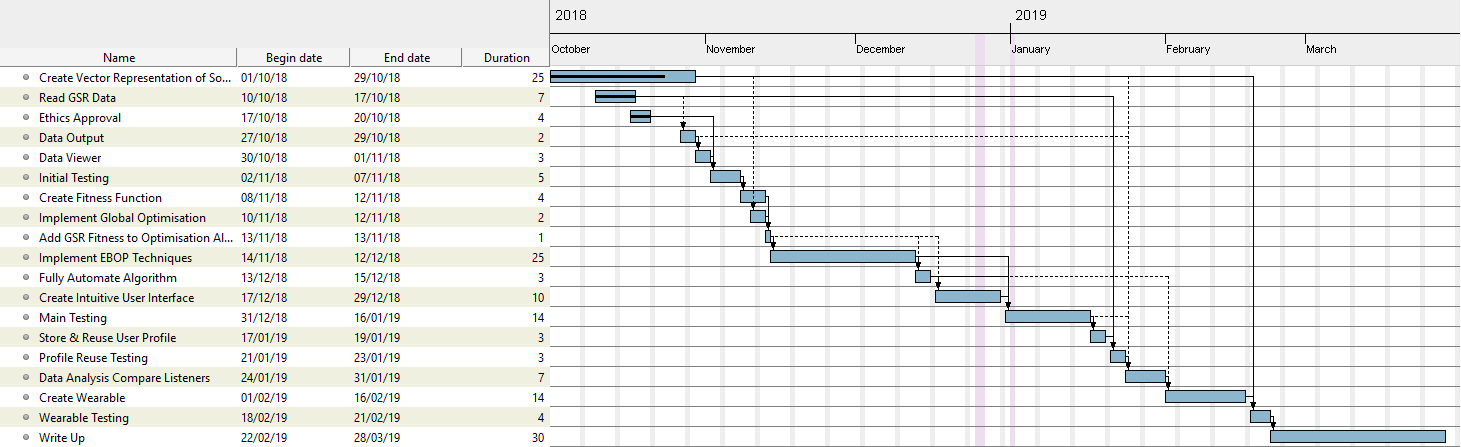
\includegraphics[width=0.9\paperwidth]{gantt}}
	
	\bibliography{document}
\end{document}